\documentclass[10pt]{article}

% Packages and macros go here
\usepackage[T1]{fontenc}
\usepackage{lmodern}
\usepackage[utf8]{inputenc}
\usepackage{microtype}
\usepackage{framed}
\usepackage{listings}
\usepackage{vmargin}
\usepackage{setspace}
\usepackage{mathrsfs, mathenv}
\usepackage{amsmath, amsthm, amssymb, amsfonts, amscd}
\usepackage{graphicx}
\usepackage{epstopdf}
\usepackage[svgnames]{xcolor}
\usepackage{hyperref}
\hypersetup{citecolor=blue, colorlinks=true, linkcolor=black}
%\usepackage[capitalise]{cleveref}
\setlength{\parskip}{6pt}
\setlength\parindent{0pt}
\usepackage{subcaption}
\usepackage{bbm}
\usepackage{cite}
\usepackage{verbatim}
\usepackage{pgfplots}
\usepackage{tikz}
\usetikzlibrary{arrows,decorations.pathmorphing,backgrounds,positioning,fit,matrix}
\usepackage{etoolbox}
\usepackage{color}
\usepackage{lipsum}
\usepackage{ifthen}
\usepackage[ruled, vlined]{algorithm2e}
\usepackage[title]{appendix}

%\usepackage[capitalise]{cleveref}
%\crefname{algocf}{Algorithm}{Algorithms}

\theoremstyle{plain}
\newtheorem{theorem}{Theorem}[section]
\newtheorem{corollary}[theorem]{Corollary}
\newtheorem{lemma}[theorem]{Lemma}
\newtheorem{proposition}[theorem]{Proposition}
\numberwithin{equation}{section}

\theoremstyle{definition}
\newtheorem{definition}{Definition}

\theoremstyle{remark}
\newtheorem{remark}[theorem]{Remark}
\newtheorem{assumption}[theorem]{Assumption}
\newtheorem{example}[theorem]{Example}


\ifpdf
  \DeclareGraphicsExtensions{.eps,.pdf,.png,.jpg}
\else
  \DeclareGraphicsExtensions{.eps}
\fi

\usepackage{mathtools}
\mathtoolsset{showonlyrefs}

% basics

% tables
\usepackage{booktabs}

% plots
\usepackage{pgfplots}
\usepackage{tikz}
\usetikzlibrary{patterns,arrows,decorations.pathmorphing,backgrounds,positioning,fit,matrix}
\usepackage[labelfont=bf]{caption}
\setlength{\belowcaptionskip}{-5pt}
\usepackage{here}
\usepackage[font=normal]{subcaption}

% Prevent itemized lists from running into the left margin inside theorems and proofs
\usepackage{enumitem}
\setlist[itemize]{leftmargin=.5in}
\setlist[enumerate]{leftmargin=.5in,topsep=3pt,itemsep=3pt,label=(\roman*)}

% Add a serial/Oxford comma by default.
\newcommand{\creflastconjunction}{, and~}

% Sets running headers as well as PDF title and authors
% title and authors
\newcommand*\samethanks[1][\value{footnote}]{\footnotemark[#1]}

\newcommand{\email}[1]{\href{#1}{#1}}
\newcommand{\TheTitle}{Model Misspecification and Uncertainty Quantification \\ for Drift Estimation in Multiscale Diffusion Processes} 
\newcommand{\TheAuthors}{A. Abdulle, G. Garegnani, G. Pavliotis, A. M. Stuart}
\title{\TheTitle}
\author{Assyr Abdulle \thanks{Institute of Mathematics, École Polytechnique Fédérale de Lausanne}
		\and Giacomo Garegnani  \samethanks
		\and Grigorios A. Pavliotis \thanks{Department of Mathematics, Imperial College London}
		\and Andrew M. Stuart \thanks{Department of Computing and Mathematical Sciences, Caltech}
		\and Andrea Zanoni \samethanks[1]
}
\date{}
%\title{Caltech notes}
%\author{Giacomo Garegnani}
%\date{}

\usepackage{amsopn}
\DeclareMathOperator{\diag}{diag}
\DeclarePairedDelimiter{\ceil}{\left\lceil}{\right\rceil}
\DeclarePairedDelimiter{\floor}{\lfloor}{\rfloor}
\newcommand{\abs}[1]{\left\lvert#1\right\rvert}
\newcommand{\norm}[1]{\left\|#1\right\|}
\renewcommand{\phi}{\varphi}
\renewcommand{\theta}{\vartheta}
\renewcommand{\Pr}{\mathbb{P}}
\newcommand{\btilde}{\widetilde}
\newcommand{\bhat}{\widehat}
\newcommand{\eqtext}[1]{\ensuremath{\stackrel{#1}{=}}}
\newcommand{\leqtext}[1]{\ensuremath{\stackrel{#1}{\leq}}}
\newcommand{\iid}{\ensuremath{\stackrel{\text{i.i.d.}}{\sim}}}
\newcommand{\totext}[1]{\ensuremath{\stackrel{#1}{\to}}}
\newcommand{\rightarrowtext}[1]{\ensuremath{\stackrel{#1}{\longrightarrow}}}
\newcommand{\leftrightarrowtext}[1]{\ensuremath{\stackrel{#1}{\longleftrightarrow}}}
\newcommand{\pdv}[2]{\ensuremath\partial_{#2}#1}
\newcommand{\N}{\mathbb{N}}
\newcommand{\R}{\mathbb{R}}
\newcommand{\C}{\mathbb{C}}
\newcommand{\OO}{\mathcal{O}}
\newcommand{\epl}{\varepsilon}
\newcommand{\diffL}{\mathcal{L}}
\newcommand{\defeq}{\coloneqq}
\newcommand{\eqdef}{\eqqcolon}
\newcommand{\Var}{\operatorname{Var}}
\newcommand{\E}{\operatorname{\mathbb{E}}}
\newcommand{\PP}{\operatorname{\mathbb{P}}}
\newcommand{\MSE}{\operatorname{MSE}}
\newcommand{\trace}{\operatorname{tr}}
\newcommand{\MH}{\mathrm{MH}}
\newcommand{\ttt}{\texttt}
\newcommand{\Hell}{d_{\mathrm{Hell}}}
\newcommand{\sksum}{{\textstyle\sum}}
\renewcommand{\d}{\mathrm{d}}
\newcommand{\dd}{\,\mathrm{d}}
\definecolor{shade}{RGB}{100, 100, 100}
\definecolor{bordeaux}{RGB}{128, 0, 50}
\newcommand{\corr}[1]{{\color{red}#1}}
\newcommand{\Tau}{\tau}
\newcommand{\LL}{L}
\newcommand{\HH}{H}
\newcommand{\WW}{W}
\newcommand{\mbf}{\mathbf}
\newcommand{\bfs}{\boldsymbol}
\newcommand{\todo}{{\color{red} TO DO}}
\newcommand{\X}{\mathbb{X}}
\newcommand{\nablar}{\nabla_{\hat x}}
\newcommand{\eval}[1]{\bigr\rvert_{#1}}
\newcommand{\normm}[1]{\norm{#1}_a}
%\newcommand{\normm}[1]{{\left\vert\kern-0.25ex\left\vert\kern-0.25ex\left\vert #1 
%		\right\vert\kern-0.25ex\right\vert\kern-0.25ex\right\vert}}
\newcommand{\gausspdf}[3]{\exp\left\{-\frac{(#1 - #2)^2}{#3}\right\}}

\usepackage[usestackEOL]{stackengine}
\newcommand\fop[3][9pt]{\mathop{\ensurestackMath{\stackengine{#1}%
			{\displaystyle#2}{\scriptstyle#3}{U}{c}{F}{F}{L}}}\limits}
\newcommand\finf[2][9pt]{\fop[#1]{\inf}{#2}}
\newcommand\fsum[2][14pt]{\fop[#1]{\sum}{#2}}
\newcommand{\prior}{p_{\mathrm{pr}}}

\definecolor{leg1}{RGB}{0,114,189}
\definecolor{leg2}{RGB}{217,83,25}
\definecolor{leg3}{RGB}{237,177,32}
\definecolor{leg4}{RGB}{126,47,142}
\definecolor{leg5}{RGB}{119,172,48}

\definecolor{leg21}{RGB}{62,38,169}
\definecolor{leg22}{RGB}{46,135,247}
\definecolor{leg23}{RGB}{55,200,151}
\definecolor{leg24}{RGB}{254,195,56}


\ifpdf
\hypersetup{
	pdftitle={\TheTitle},
	pdfauthor={\TheAuthors}
}
\fi


\begin{document}

\subsection{Central limit theorem}

\corr{Text to be added with motivation, proof in Appendix \ref{ap:CLT}.
	\begin{theorem}\label{thm:CLT} Central limit theorem statement:
		\begin{equation}
		\lim_{\epl \to 0}\lim_{T \to \infty} \sqrt{T}\left(\widehat A^\epl_k(T) - A\right) = \Lambda, \quad \text{in law,}
		\end{equation}
		where $\Lambda \sim \mathcal N(0, \Gamma)$ and
		\begin{equation}
		\Gamma = 2\sigma \E^{\rho^0}[V'(Z) \otimes V'(X)]^{-1}\E^{\rho^0}[V'(Z) \otimes V'(Z)]\E^{\rho^0}[V'(X) \otimes V'(Z)]^{-1}.
		\end{equation}
		This covariance may not be correct (see proof in the Appendix) but it is just the limit of the ``third term'' 
	\end{theorem}
}



\subsection{Central limit theorem}
\begin{figure}[t]
	\centering
	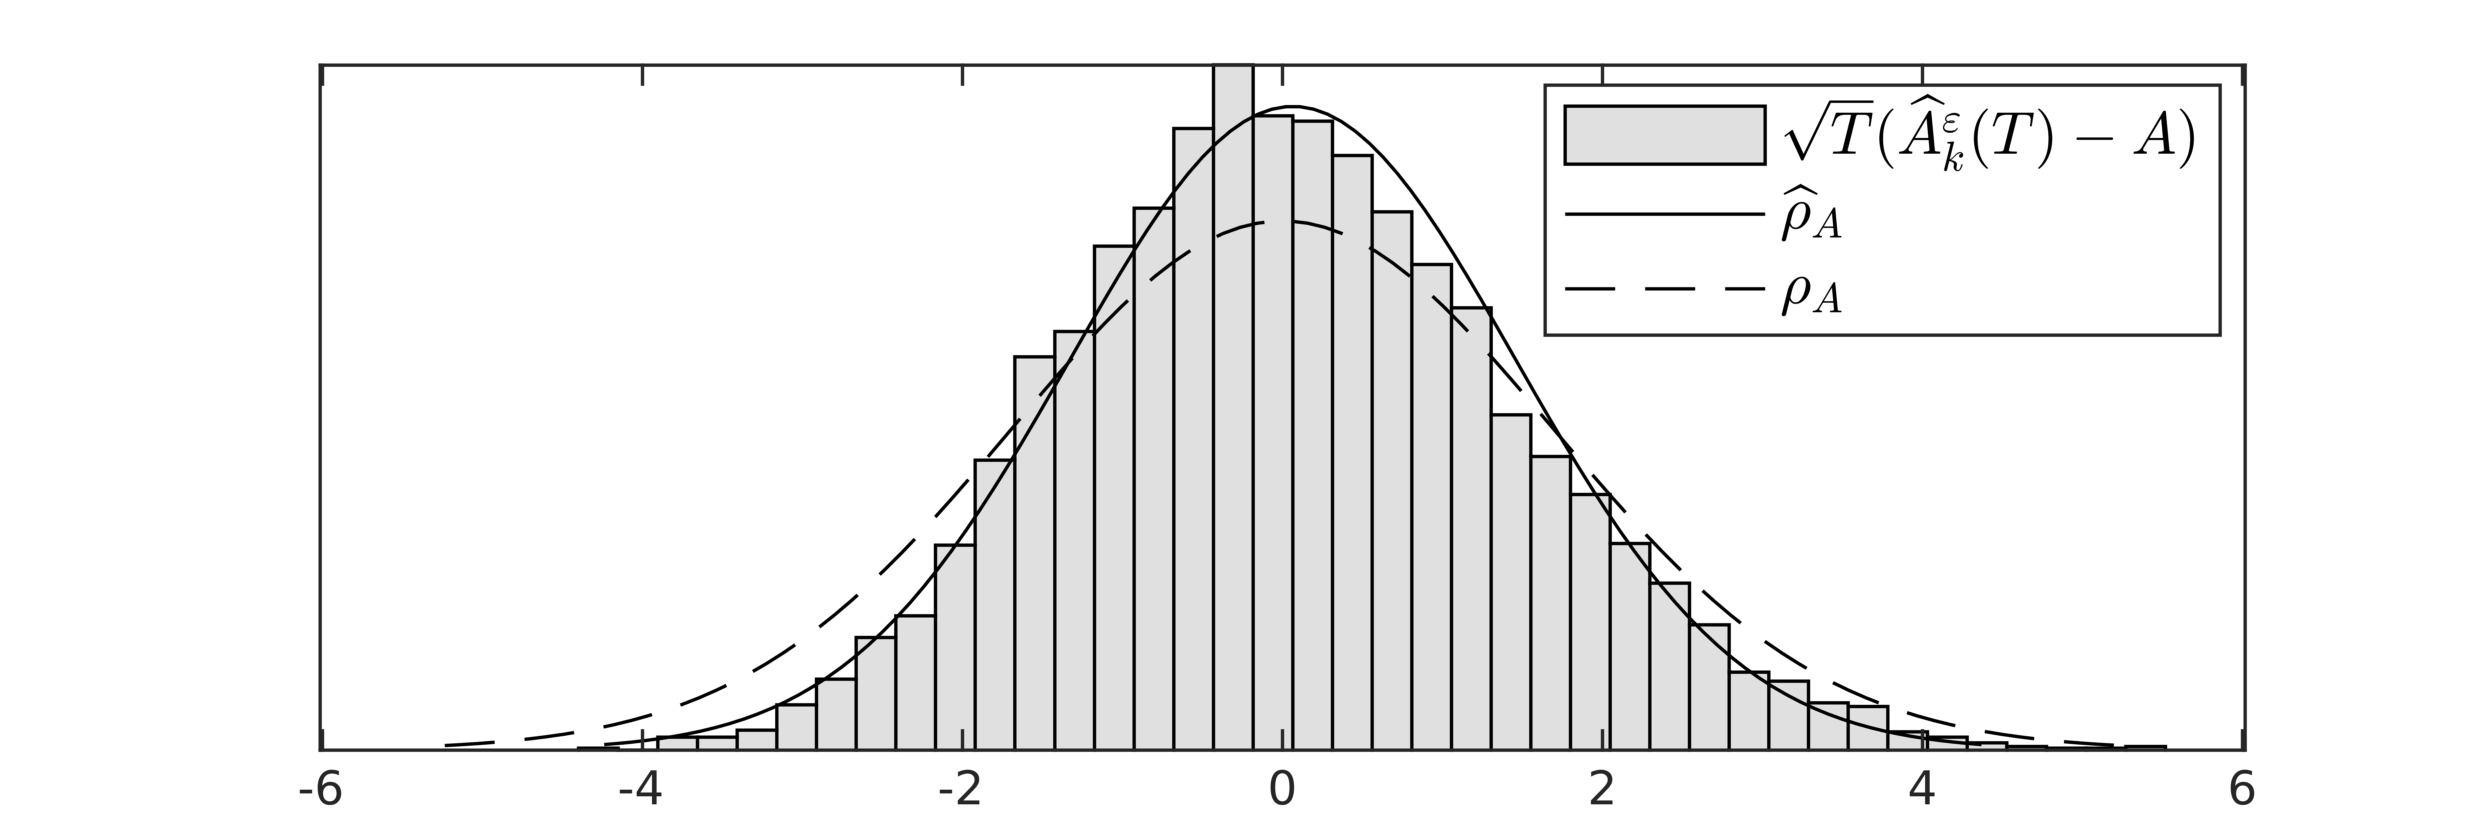
\includegraphics[]{../Figures/CLT}
	\caption{Central limit theorem result. The histogram represents numerical results, the solid curve a Gaussian fit to the latter and the dashed curve the theoretical estimate given in Theorem \ref{thm:CLT}.}
	\label{fig:CLT}
\end{figure}

In this experiment we wish to confirm the validity of Theorem \ref{thm:CLT}. We consider the same test equation as for Section \ref{sec:Num_Param}, i.e., the quadratic potential $V(x) = x^2/2$ with fluctuating potential $p(y) = \sin(y)$, multiscale parameter $\epl = 0.05$ and diffusion coefficient $\sigma = 1$. The parameters of the filter are set to $\beta = 1$ and $\delta = 1$. We compute the estimator $\widehat A^\epl_k(T)$ with final time $T = 10^3$ on $2000$ realizations of the solution and estimate the quantity 
\begin{equation}	
\Delta_A^\epl(T) \defeq \sqrt{T}\left(\widehat A^\epl_k(T) - A\right),	
\end{equation}
where $A$ is the drift coefficient of the homogenized equation. Results, depicted in Figure \ref{fig:CLT}, show that the distribution of $\Delta_A^\epl(T)$ indeed follows a zero-mean Gaussian law, \corr{whose covariance agrees with the theoretical results (?)}.


\section{Proof of Theorem \ref{thm:CLT}}\label{ap:CLT}

Let us first introduce a technical Lemma.
\begin{lemma}\label{lem:CLT} Let $\mathcal L_\epl$ be the generator of the couple $(X^\epl, Z^\epl)^\top$, i.e.,
	\begin{equation}
		\mathcal L_\epl = -\left(\alpha \cdot V'(x) + \frac1\epl p'\left(\frac{x}{\epl}\right)\right)\partial_x + \frac1\delta (x - z) \partial_z  + \sigma \partial^2_{xx}.
	\end{equation} 
	Moreover, let $\rho^\epl$ be the density of the invariant measure of $(X^\epl, Z^\epl)^\top$ and $u^\epl\colon \R^2 \to \R^N$ be the solution of 
	\begin{equation}\label{eq:CLT_Poisson}
		-\mathcal L_\epl u^\epl = \chi^\epl -  \E^{\rho^\epl}[\chi^\epl(X^\epl, Z^\epl)],
	\end{equation}
	satisfying $\E^{\rho^\epl}[u^\epl(X^\epl, Z^\epl)] = 0$ for $\chi^\epl \colon \R^2 \to \R^N$. Then, it holds
	\begin{equation}\label{eq:CLT_PoissonIto}
		\frac{1}{T} \int_0^T  \chi^\epl(X_t^\epl, Z_t^\epl) \dd t = \E^{\rho^\epl}[\chi^\epl(X^\epl, Z^\epl)] - \frac{R^\epl(T)}{T} + \sqrt{2\sigma}\frac{S^\epl(T)}{T},
	\end{equation}
	where
	\begin{equation}\label{eq:CLT_PoissonRemainders}
		R^\epl(T) \defeq u^\epl(X^\epl_T, Z^\epl_T) - u^\epl(X^\epl_0, Z^\epl_0), \quad S^\epl(T) \defeq \int_0^T \partial_x u^\epl(X_t^\epl, Z_t^\epl) \dd W_t.
	\end{equation}
	Moreover, it holds
	\begin{equation}\label{eq:CLT_Equiv}
		2\sigma \E^{\rho^\epl}[\partial_x u^\epl(X^\epl, Z^\epl) \otimes \partial_x u^\epl(X^\epl, Z^\epl)] = \E^{\rho^\epl}
		\begin{aligned}[t]
		[&\chi^\epl(X^\epl, Z^\epl) \otimes u^\epl(X^\epl, Z^\epl) \\
		&+ u^\epl(X^\epl, Z^\epl) \otimes \chi^\epl(X^\epl, Z^\epl)].
		\end{aligned}
	\end{equation}	
\end{lemma}
\begin{proof} The proof of \eqref{eq:CLT_PoissonIto} and \eqref{eq:CLT_PoissonRemainders} is an application of the Itô formula (see e.g. \cite[Remark 6.17]{PaS08}). For \eqref{eq:CLT_Equiv}, it is possible to show that since $\mathcal L_\epl^*\rho^\epl = 0$ it holds 
	\begin{equation}
		\mathcal L_\epl^* (u^\epl \rho^\epl) = 2 \sigma \rho^\epl \partial_{xx}^2 u^\epl - \rho^\epl \mathcal L_\epl u^\epl + 2 \sigma \partial_x u^\epl \partial_x \rho^\epl.
	\end{equation}
	Therefore, an integration by parts yields 
	\begin{equation}
	\begin{aligned}
		\E^{\rho^\epl}[\mathcal L_\epl u^\epl(X^\epl, Z^\epl) \otimes u^\epl(X^\epl, Z^\epl)] &= 	\int_{\R}\int_{\R} u^\epl \otimes \mathcal L_\epl^*\left(u^\epl \rho^\epl\right) \dd x \dd z \\
		&= -\int_{\R}\int_{\R}u^\epl \otimes \mathcal L_\epl u^\epl \rho^\epl \dd x \dd z- 2\sigma \int_{\R}\int_{\R} \partial_x u^\epl \otimes \partial_x u^\epl \rho^\epl \dd x \dd z\\
		&= 
		\begin{aligned}[t]
		&-\E^{\rho^\epl}[u^\epl(X^\epl, Z^\epl) \otimes \mathcal L_\epl u^\epl(X^\epl, Z^\epl)] \\
		&- 2\sigma \E^{\rho^\epl}[\partial_x u^\epl(X^\epl, Z^\epl) \otimes \partial_x u^\epl(X^\epl, Z^\epl)].
		\end{aligned}
	\end{aligned}
	\end{equation}
	Finally, since $\E^{\rho^\epl}[u(X^\epl, Z^\epl)] = 0$ 
	\begin{equation}
	\begin{aligned}
		2\sigma \E^{\rho^\epl}[\partial_x u^\epl(X^\epl, Z^\epl) \otimes \partial_x u^\epl(X^\epl, Z^\epl)] &= -\E^{\rho^\epl}
		\begin{aligned}[t]
		[&\mathcal L_\epl u^\epl(X^\epl, Z^\epl) \otimes u^\epl(X^\epl, Z^\epl) \\
		& + u^\epl(X^\epl, Z^\epl) \otimes \mathcal L_\epl u^\epl(X^\epl, Z^\epl)]
		\end{aligned}
		\\
		&= \E^{\rho^\epl}
		\begin{aligned}[t]
		[&\chi^\epl(X^\epl, Z^\epl) \otimes u^\epl(X^\epl, Z^\epl) \\
		&+ u^\epl(X^\epl, Z^\epl) \otimes \chi^\epl(X^\epl, Z^\epl)],
		\end{aligned}
	\end{aligned}
	\end{equation}
	which is the desired result.
\end{proof}

\begin{lemma} \label{lem:CLT_hom}
	Let $u^\epl$ be the solution of \eqref{eq:CLT_Poisson} with 
	\begin{equation}
		\chi^\epl(x, z) = \frac 1 \epl p' \left ( \frac x \epl \right ) V'(z) - V'(z) \otimes V'(x) \mathcal M_\epl^{-1} \mathfrak p_\epl,
	\end{equation}
	where
	\begin{equation}
		\mathcal M_\epl \defeq \E^{\rho^\epl} [ V'(Z^\epl) \otimes V'(X^\epl) ], \quad \mathfrak p_\epl \defeq \E^{\rho^\epl} \left [ \frac{1}{\epl} p' \left ( \frac{X^\epl}{\epl} \right ) V'(Z^\epl) \right ].
	\end{equation}
	Then, $u^\epl \to 0$ \corr{in which sense?} for $\epl \to 0$.
\end{lemma}
\begin{proof} We here present a formal proof based on asymptotic expansion with respect to $\epl$. Let us first remark that by definition
	\begin{equation}
		\E^{\rho^\epl}[\chi^\epl(X^\epl, Z^\epl)] = 0,
	\end{equation}
	and therefore problem \eqref{eq:CLT_Poisson} reads
	\begin{equation}
		-\mathcal L^\epl u^\epl = \chi^\epl.
	\end{equation}
	Let us now denote $y = x/\epl$ and write
	\begin{equation}
		u^\epl(x, z) = u_0(x, y, z) + \epl u_1(x, y, z) + \epl^2 u_2(x, y, z) + \ldots,
	\end{equation}
	which implies that
	\begin{equation}
	\begin{aligned}
		\partial_x u^\epl &= \partial_x(u_0(x, y, z) + \epl u_1(x, y, z) + \epl^2 u_2(x, y, z) + \ldots) \\
		&\quad+ \frac1\epl\partial_y(u_0(x, y, z) + \epl u_1(x, y, z) + \epl^2 u_2(x, y, z) + \ldots).
	\end{aligned}
	\end{equation}
	Let us first remark that from the proof of Theorem \ref{thm:mainTheorem} we have that
	\begin{equation}
		\lim_{\epl \to 0} \mathcal M_\epl^{-1}\mathfrak p_\epl = A - \alpha.
	\end{equation} 	
	Replacing $u^\epl$ in \eqref{eq:CLT_Poisson} and grouping the terms of order $\epl^0$, $\epl^{-1}$ and $\epl^{-2}$ we get the system
	\begin{align}
		L_0 u_0 &= 0, \label{eq:CLT_AsExp1}\\
		L_1 u_0 + L_0 u_1 &= - p'(y) V'(z), \label{eq:CLT_AsExp2}\\
		L_0 u_2 + L_1 u_1 + L_2 u_0 &= \left(V'(z) \otimes V'(x)\right) (A - \alpha),\label{eq:CLT_AsExp3}
	\end{align}
	where 
	\begin{equation}
	\begin{aligned}
		L_0 &= -p'(y) \partial_y + \sigma \partial^2_{yy},\\
		L_1 &= -p'(y) \partial_x - \alpha \cdot V'(x) \partial_y + 2 \sigma \partial^2_{xy}, \\
		L_2 &= 	-\alpha \cdot V'(x) \partial_x - \frac1{\delta}(z - x)	\partial_z + \sigma \partial^2_{xx}.
	\end{aligned}
	\end{equation}
	Let us first remark that equation \eqref{eq:CLT_AsExp1} is satisfied for $u_0 = u_0(x, z)$ independent of $y$. In particular, the kernel of $L_0$ is made of constants and the kernel of $L_0^*$ is one-dimensional and $\mathrm{Ker}(L_0^*) = \mathrm{Span}\{\rho\}$ where
	\begin{equation}\label{eq:CLT_Invariant}
		\rho(y) = \frac1Z e^{-p(y)/\sigma}, \quad\text{where}\quad Z = \int_0^L e^{-p(y)/\sigma} \dd y,
	\end{equation} 
	where $L$ is the period of $p$. Since $u_0$ is independent of $y$ equation \eqref{eq:CLT_AsExp2} reduces to 
	\begin{equation}
		L_0 u_1 = p'(y)\left(\partial_x u_0 -V'(z)\right).
	\end{equation}
	Let us remark that the general solution $u_1$ can be written as
	\begin{equation}
		u_1(x,y,z) = \Phi(y)\left(\partial_x u_0(x, z) - V'(z)\right),
	\end{equation}
	where $\Phi \colon \R \to \R$ satisfies
	\begin{equation}
		-L_0 \Phi = -p'(y).
	\end{equation} 
	Let us remark that this cell problem is the same as \eqref{eq:CellProblem}. We consider now equation \eqref{eq:CLT_AsExp3} and remark that we can rewrite it as
	\begin{equation}
	\begin{aligned}
		L_0 u_2 &= (V'(z) \otimes V'(x))(A - \alpha) - \left(2\Phi'(y) - \frac1\sigma p'(y) \Phi(y) + 1\right) \sigma \partial^2_{xx}u_0 \\
		&\quad +\left(\Phi'(y) + 1\right) \left( \alpha \cdot V'(x) \right) \partial_x u_0 - \left(V'(z) \otimes V'(x) \right)\alpha \Phi'(y) + \frac1\delta(z-x) \partial_z u_0.
	\end{aligned}
	\end{equation}
	By the Fredholm alternative, in order for \eqref{eq:CLT_AsExp3} to have a solution we need the right hand side to have zero-mean with respect to $\rho$ in \eqref{eq:CLT_Invariant}. Therefore, recalling that the homogenization coefficient $K$ in \eqref{eq:K_HOM} is given by
	\begin{equation}
		K = \int_0^L (1 + \Phi'(y))^2 \rho(y) \dd y
	\end{equation}
	and remarking that integrations by part allow to rewrite $K$ as
	\begin{equation}
		K = \int_0^L (1 + \Phi'(y)) \rho(y) \dd y, \quad  K = \int_0^L \left(2\Phi'(y) - \frac1\sigma p'(y) \Phi(y) + 1\right) \rho(y) \dd y,
	\end{equation}
	we get
	\begin{equation}
		0 = (V'(z) \otimes V'(x))(A - \alpha - (K - 1)\alpha) - K \sigma \partial^2_{xx}u_0 + \left(K \alpha \cdot V'(x)\right) \partial_x u_0  + \frac1\delta(z-x) \partial_z u_0.
	\end{equation}
	Moreover, since $A = K\alpha$ and $\Sigma = K\sigma$, it implies
	\begin{equation}
		0 = -\Sigma \partial^2_{xx}u_0 + \left(A \cdot V'(x)\right) \partial_x u_0  + \frac1\delta(z-x) \partial_z u_0,
	\end{equation}
	which can be written as
	\begin{equation}\label{eq:CLT_Poisson_hom}
		- \mathcal L_0 u_0 = 0,
	\end{equation}
	where $\mathcal L_0$ is the generator of the couple $(X^0,Z^0)^\top$. Finally, the unique solution of \eqref{eq:CLT_Poisson_hom} satisfying
	\begin{equation}
		\E^{\rho^0}[u_0(X,Z)] = 0,
	\end{equation}
	is given by
	\begin{equation}
		u_0(x,z) = 0.
	\end{equation}
\end{proof}

We can now proceed with the main proof.
\begin{proof}[Proof of Theorem \ref{thm:CLT}] Let us introduce the notation
	\begin{equation}\label{eq:CLT_DefMEps}
	\mathcal M_\epl \defeq \E^{\rho^\epl} [ V'(Z^\epl) \otimes V'(X^\epl) ], \quad \mathcal M_0 \defeq \E^{\rho^0} [ V'(Z) \otimes V'(X) ],
	\end{equation}
	and the notation
	\begin{equation}
	\mathfrak p_\epl \defeq \E^{\rho^\epl} \left [ \frac{1}{\epl} p' \left ( \frac{X^\epl}{\epl} \right ) V'(Z^\epl) \right ]
	\end{equation}
	and let us remark that from the proof of Theorem \ref{thm:mainTheorem} one can deduce the equalities
	\begin{equation}\label{eq:CTL_A}
	A = \frac1\delta \mathcal M_0^{-1} \E^{\rho^0}[(X - Z)^2 V''(Z)],
	\end{equation}
	and
	\begin{equation}\label{eq:CTL_alpha}
	\alpha = \mathcal M_\epl^{-1} \left(\frac1\delta \E^{\rho^\epl}[(X^\epl - Z^\epl)^2 V''(Z^\epl)] - \mathfrak p_\epl \right).
	\end{equation}
	Let us furthermore remark that the decomposition \eqref{eq:alphaDecomposition} yields
	\begin{equation}
	\sqrt{T}\left(\widehat A^\epl_k(T) - A\right) = \sqrt{T} \left(\alpha - A + I_1^\epl - I_2^\epl\right).
	\end{equation}
	Replacing the expression for $A$ and $\alpha$ given in \eqref{eq:CTL_A} and \eqref{eq:CTL_alpha}, we get
	\begin{equation}
	\begin{aligned}
	\sqrt{T}\left(\widehat A^\epl_k(T) - A\right) &= \sqrt{T}\left( I_1^\epl(T) - \mathcal M_\epl^{-1} \mathfrak p_\epl \right) \\
	&+  \frac{\sqrt{T}}\delta \left( \mathcal M_\epl^{-1} \E^{\rho^\epl}[(X^\epl - Z^\epl)^2 V''(Z^\epl)] - \mathcal M_0^{-1} \E^{\rho^0}[(X - Z)^2 V''(Z)] \right) \\
	&- \sqrt{T} I_2^\epl(T).
	\end{aligned}
	\end{equation}
	\corr{Third term is OK:} We rewrite the term involving $I_2^\epl(T)$ as
	\begin{equation}
	\sqrt{T} I_2^\epl(T) = \frac{\sqrt{2\sigma}}{\sqrt{T}} \widetilde M^{-1} Q^\epl(T),
	\end{equation}
	where, since $Z_t^\epl$ is adapted with respect to the natural filtration $\mathcal F_t$ of the Wiener process $W \defeq \left(W_t, t \geq 0\right)$, the quantity
	\begin{equation}
	Q^\epl(T) \defeq \int_0^T V'(Z^\epl_t) \dd W_t,
	\end{equation}
	is a martingale whose quadratic variation is given by
	\begin{equation}
	\langle Q^\epl \rangle_T = \int_0^T V'(Z^\epl_t) \otimes V'(Z^\epl_t) \dd t. 
	\end{equation}
	Since the ergodic theorem guarantees that 
	\begin{equation}
	\lim_{T\to\infty}\frac{\langle Q^\epl \rangle_T}{T} = \E^{\rho^\epl}[V'(Z^\epl) \otimes V'(Z^\epl)], \quad \text{in } L^1(\mu^\epl),
	\end{equation}
	the martingale central limit theorem gives 
	\begin{equation}
	\lim_{T\to\infty}\frac{1}{\sqrt{T}} Q^\epl(T) = \Xi^\epl, \quad \text{in law},
	\end{equation}
	where $\Xi^\epl \sim \mathcal N(0, \E^{\rho^\epl}[V'(Z^\epl) \otimes V'(Z^\epl)])$.
	Now, by the ergodic theorem 
	\begin{equation}
	\lim_{T \to \infty} \widetilde M^{-1} = \mathcal M_\epl^{-1}, \quad \text{a.s.}
	\end{equation}
	Therefore, we have by Slutsky's theorem that
	\begin{equation}
	\lim_{T \to \infty} \sqrt{T} I_2^\epl(T) = \Lambda^\epl \sim \mathcal N\left(0, \Gamma^\epl\right), \quad \text{in law}.
	\end{equation}
	where the covariance matrix $\Gamma^\epl$ is given by
	\begin{equation}
	\Gamma^\epl = 2\sigma \mathcal M_\epl^{-1}\E^{\rho^\epl}[V'(Z^\epl) \otimes V'(Z^\epl)]\mathcal M_\epl^{-\top}.
	\end{equation}
	Finally, we denote by $\Lambda$ the limit for $\epl \to 0$ of the sequence of Gaussian random variables $\Lambda^\epl$.
	
	\corr{Idea for the first term:} Let us introduce the notation
	\begin{equation}
	J_1^\epl(T) \defeq \sqrt{T}\left( I_1^\epl(T) - \mathcal M_\epl^{-1} \mathfrak p_\epl\right),
	\end{equation}
	and let us remark that we can rewrite
	\begin{equation} \label{eq:decomposition_first_term}
	\begin{aligned}
	J_1^\epl(T) = \sqrt{T} &\left(\frac1T \int_0^T V'(Z^\epl_t) \otimes V'(X^\epl_t) \dd t\right)^{-1}\\
		&\quad \times \left(\frac1T \int_0^T \left( \frac{1}{\epl} p' \left ( \frac{X^\epl_t}{\epl} \right ) V'(Z^\epl_t)	- V'(Z^\epl_t) \otimes V'(X^\epl_t) \mathcal M_\epl^{-1} \mathfrak p_\epl \right) \dd t	 \right).
	\end{aligned}
	\end{equation}
	Let us denote by $u^\epl$ the solution of \eqref{eq:CLT_Poisson} with right hand side
	\begin{equation}
	\chi^\epl(x, z) = \frac 1 \epl p' \left ( \frac x \epl \right ) V'(z) - V'(z) \otimes V'(x) \mathcal M_\epl^{-1} \mathfrak p_\epl,
	\end{equation}
	and note that $\E^{\rho^\epl}[\chi^\epl(X^\epl,Z^\epl)] = 0$. Then, by Lemma \ref{lem:CLT}, we have
	\begin{equation}
	J_1^\epl(T)= \sqrt{T} \left(\frac1T \int_0^T V'(Z^\epl_t) \otimes V'(X^\epl_t) \dd t\right)^{-1} \left( -\frac{R^\epl(T)}{T} + \sqrt{2\sigma}\frac{S^\epl(T)}{T} \right),
	\end{equation}
	where $R^\epl(T)$ and $S^\epl(T)$ are defined in \eqref{eq:CLT_PoissonRemainders}. Since \corr{$R^\epl(T)$ is bounded independently of $\epl$ (is it clear?)}, we first get by the ergodic theorem
	\begin{equation}
	\lim_{T \to \infty} \left(\frac1T \int_0^T V'(Z^\epl_t) \otimes V'(X^\epl_t) \dd t\right)^{-1} \frac{R^\epl(T)}{\sqrt{T}} = 0, \quad \text{a.s.}
	\end{equation}
	Repeating the same reasoning as for $Q^\epl(T)$ and employing the ergodic theorem and the Slutsky's theorem, we get 
	\begin{equation}
	\lim_{T \to \infty} J_1^\epl(T) = \lim_{T \to \infty} \sqrt{2\sigma} \left(\frac1T \int_0^T V'(Z^\epl_t) \otimes V'(X^\epl_t) \dd t\right)^{-1} \frac{S^\epl(T)}{\sqrt{T}} = \Lambda_1^\epl \sim \mathcal N(0, \Gamma_1^\epl),
	\end{equation}
	where the covariance is given by due to \eqref{eq:CLT_Equiv}
	\begin{equation}
	\begin{aligned}
	\Gamma_1^\epl &= 2\sigma \mathcal M_\epl^{-1}\E^{\rho^\epl}[\partial_x u^\epl(X^\epl, Z^\epl) \otimes \partial_x u^\epl(X^\epl, Z^\epl)]\mathcal M_\epl^{-\top} \\
	&= \mathcal M_\epl^{-1}\E^{\rho^\epl}[u^\epl(X^\epl, Z^\epl) \otimes \chi^\epl(X^\epl, Z^\epl) + \chi^\epl(X^\epl, Z^\epl) \otimes u^\epl(X^\epl, Z^\epl)]\mathcal M_\epl^{-\top}.
	\end{aligned}
	\end{equation}
	\corr{For the covariance $\Gamma_1^\epl$ we don't know how it behaves in the limit $\epl \to 0$. It would be nice if it was vanishing since it involves the solution $u^\epl$, which goes to zero (in some sense) due to Lemma \ref{lem:CLT_hom}.}
	
	\corr{Idea for the second term:} Let us now introduce the notation
	\begin{equation}
		J_2^\epl(T) = \frac{\sqrt{T}}\delta \left( \mathcal M_\epl^{-1} \E^{\rho^\epl}[(X^\epl - Z^\epl)^2 V''(Z^\epl)] - \mathcal M_0^{-1} \E^{\rho^0}[(X - Z)^2 V''(Z)] \right).
	\end{equation}
	We have the decomposition
	\begin{equation}
	\begin{aligned}
	J^\epl_{2}(T) &=  \frac{\sqrt{T}}\delta \left( \mathcal M_\epl^{-1}  - \mathcal M_0^{-1} \right)\E^{\rho^\epl}[(X^\epl - Z^\epl)^2 V''(Z^\epl)] \\
	&\quad + \frac{\sqrt{T}}\delta \mathcal M_0^{-1}\left(\E^{\rho^\epl}[(X^\epl - Z^\epl)^2 V''(Z^\epl)] - \E^{\rho^0}[(X - Z)^2 V''(Z)] \right) \\
	&\eqdef J_{2,1}^\epl(T) + J_{2,2}^\epl(T).
	\end{aligned}
	\end{equation}
	\corr{In order to send the terms above to zero, we need the convergence rate of $\mu^\epl$ to $\mu^0$ w.r.t. $\epl$ (by fixing $T = \epl^{-\gamma}$ with an appropriate $\gamma$). Some arguments in this sense seem to appear in [\textit{Periodic Homogenization for Hypoelliptic Diffusions} -- M. Hairer and G.A. Pavliotis 2004] but it is not clear to us whether it applies to this case too.}
\end{proof}

\end{document}